\section{Integrais simples em coordenadas polares}
\label{sec:int1polar}

O problema do cálculo de áreas examinado na
seção~\ref{sec:revisao-int1}, com coordenadas retangulares, tem um
equivalente em coordenadas polareas, ou seja: dada uma equação polar
qualquer $r = f(\theta)$, como encontrar a área da região $R$
delimitada pelos ângulos $\theta = a$ e $\theta = b$
(figura~\ref{fig:areapolar1})?

\begin{figure}[H]
  \begin{center}
    \caption{O problema da área em coordenadas polares}
    \label{fig:areapolar1}
    \fbox{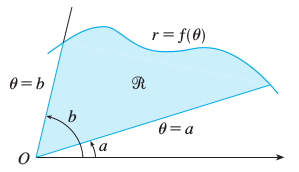
\includegraphics[scale=0.7]{imagens/int26.png}}\\
    \footnotesize{James Stewart: \emph{Cálculo} (8ª ed.,\ vol.\ 2, pg.\ 606)}
  \end{center}
\end{figure}

A solução é dividir a região $R$ em vários setores, calcular a área de
cada setor e somar todas as áreas (figura~\ref{fig:areapolar2}), de
forma análoga ao procedimento para o cálculo de áreas em coordenadas
retangulares:

\begin{figure}[H]
  \begin{center}
    \caption{Divisão da região $R$ em vários setores}
    \label{fig:areapolar2}
    \fbox{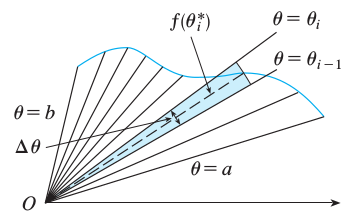
\includegraphics[scale=0.6]{imagens/int27.png}}\\
    \footnotesize{James Stewart: \emph{Cálculo} (8ª ed.,\ vol.\ 2, pg.\ 606)}
  \end{center}
\end{figure}

Sabemos que a área de um setor de um círculo é proporcional ao
ângulo $\theta$ (figura~\ref{fig:areapolar3}) e dada por:

\begin{equation}
  \label{eq:areasetor}
  \begin{split}
    A &= \pi r^2 \times \frac{\theta}{2\pi}\\
    &= \frac{1}{2}\theta r^2
  \end{split}
\end{equation}

\begin{figure}[H]
  \begin{center}
    \caption{Área de um setor de um círculo}
    \label{fig:areapolar3}
    \fbox{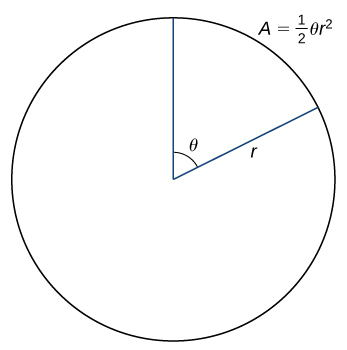
\includegraphics[scale=0.45]{imagens/int28.png}}\\
    \footnotesize{Gilbert Strang \& Edwin Herman: \emph{Calculus}
          (ed.\ online, 2017, vol.\ 2, pg.\ 663)}
    \end{center}
\end{figure}

Como o raio $r$ na equação~\ref{eq:areasetor} corresponde à
$f(\theta^*_i)$, podemos calcular a área de \emph{cada
setor} na figura~\ref{fig:areapolar2} da seguinte forma:

\begin{equation}
  \begin{split}
    \Delta A_i &\approx \frac{1}{2}\color{red}r\color{black}^2 \Delta \theta\\
        &\approx \frac{1}{2}\left[\color{red}f(\theta_i^*)\color{black}\right]^2 \Delta \theta
  \end{split}
\end{equation}

Para calcular a estimativa da área total da região $R$ sob a função $r = f(\theta)$,
delimitada pelos ângulos $\theta = a$ e $\theta =  b$, basta somar as
áreas de cada setor individual:

\begin{equation}
    A \approx \sum_i^n \frac{1}{2}\left[f(\theta_i^*)\right]^2 \Delta \theta
\end{equation}

É fácil perceber que à medida em que aumentamos o números de setores a
estimativa do cálculo da área fica mais precisa. No limite, quando o
número de setores tende ao infinito, a área tende ao valor exato, e
essa é a idéia do cálculo de áreas em coordenadas polares:

\begin{equation}
  \begin{split}
  A &= \lim_{n \to \infty} \sum_i^n
  \frac{1}{2}\left[f(\theta_i^*)\right]^2 \Delta \theta\\
  &= \int_a^b \frac{1}{2}\left[f(\theta)\right]^2 \diff \theta\\
  &= \int_a^b \frac{1}{2}r^2 \diff \theta
  \end{split}
\end{equation}
